\section{Rancangan Solusi}
\begin{figure}[h]
  \centering
  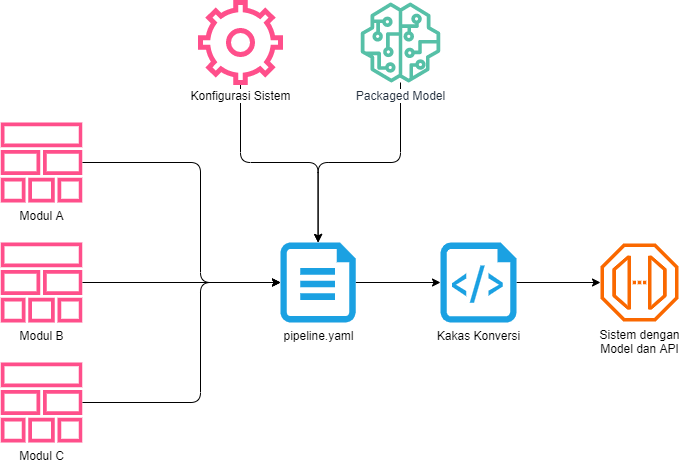
\includegraphics[width=0.8\textwidth]{03-rancangan-solusi.drawio.png}
  \caption{Rancangan Solusi (Sumber: Penulis)}
\end{figure}

Solusi yang saya tawarkan adalah membuat prototipe kakas yang dapat menganalisis suatu eksperimen dan mengubahnya menjadi suatu sistem yang koheren.
Definisi dari perjanjian data yang menjadi masukan dan keluaran akan dibuat oleh sistem secara otomatis berdasarkan eksperimen.
Alur pemrosesan yang didefinisikan dapat dibuat lewat \textit{markup} file seperti JSON atau YAML.
Alur didefinisikan lewat pemanggilan modul-modul yang diimplementasikan lebih dulu.

Modul tersebut akan diimplementasikan dalam satu bahasa pilihan, yaitu bahasa Go.
Pemilihan tersebut didasarkan karena Go adalah bahasa yang cukup fleksibel dan dalam kasus ini sekaligus digunakan untuk menguji kemampuan prototipe ini untuk diterapkan dalam bahasa yang \textit{compiled}, serta Go memiliki dukungan yang baik terhadap sistem yang berbasis modul.
Dalam proposal rancangan ini, modul-modul sederhana yang biasa digunakan akan diimplementasikan, khususnya berfokus pada data tabular.

Hasil akhir dari kakas ini adalah sebuah sistem yang siap digunakan untuk production.
Pemilihan interface untuk model ini ditentukan lewat file markup yang telah dibua.
Metode komunikasi menggunakan gRPC dan REST akan diimplementasikan sebagai contoh metode yang umum digunakan.

